% Formatting
\documentclass{scrartcl}
\usepackage{hyperref}
\usepackage{makeidx}
    \makeindex
\usepackage{xparse}

\usepackage{graphicx}
\graphicspath{ {.} }

\usepackage[most]{tcolorbox}
\NewDocumentCommand\newtcbtheoremautoindex{ O{} m  m m m }{%%
\newtcbtheorem[#1]{#2inner}{#3}{#4}{#5}%
\NewDocumentEnvironment { #2 } { s O{} m m }
{\IfBooleanTF{##1}
   {\begin{#2inner}[##2]{##3}{##4}}% not to index
   {\begin{#2inner}[##2, index={##3}]{##3}{##4}}% to index
} {\end{#2inner}}
% starred version (not labeled and not listed in lists of theorems):
\NewDocumentEnvironment { #2* } { O{} m }
   {\begin{#2inner*}[##1]{##2}}% (and no index as well)
   {\end{#2inner*}}
}%%

\newtcbtheoremautoindex[]{defi}{}{}{def}

% End formatting

% ====================
% Begin Status report!
% ====================

\begin{document}
\section*{EG-310 Weekly Status Report}
\begin{center}
    \begin{tabular}{ l l }
        Project Lead     & Joseph Sedutto          \\
        Date             & \today         \\
        Reporting Period & January 17 - Febuary 17
    \end{tabular}
\end{center}

\begin{defi}{Project Status Summary}{}
    \begin{tabular}{ l l r }
        Budget   & On Track & We have begun spending and qouting         \\
        Schedule & On Track & We are slightly behind schedule                     \\
        Scope    & On Track & We are within scope.
    \end{tabular}
\end{defi}

\begin{defi}{Work Completed this week}{}
    - Created inital frame and CAD \\
    - Completed inital revision of PCB \\
    - Completed PDR and presented \\
    - Reviewed PDR feedback and created inital CDR
\end{defi}

\begin{defi}{Open issues}{}
    % Check open issues https://github.com/KenwoodFox/EG-310-InvertedPendulum/issues
    No issues and \href{https://github.com/KenwoodFox/EG-310-InvertedPendulum/pulls}{four pull requests} are waiting for feedback or review.
\end{defi}

\begin{defi}{Todo for next week}{}
    % Check projects tab https://github.com/users/KenwoodFox/projects/1
    - Finalize PDP draft for submission on January 30, 2021.  \\ 
    - Convert PDP data into a simplistic slideshow format. \\
    - Create more sketches of subassemblies and identify subassemly requirements.
\end{defi}

\begin{defi}{Comments/Team Dynamics}{}
    - Everyone still seems cheerful!
\end{defi}


\pagebreak
\section{Meeting Notes}
% Include meeting notes verbatim
\lstinputlisting[breaklines=true]{../Meeting Minutes/Week29-17.md}

\pagebreak
\section{Releases Published This Week}

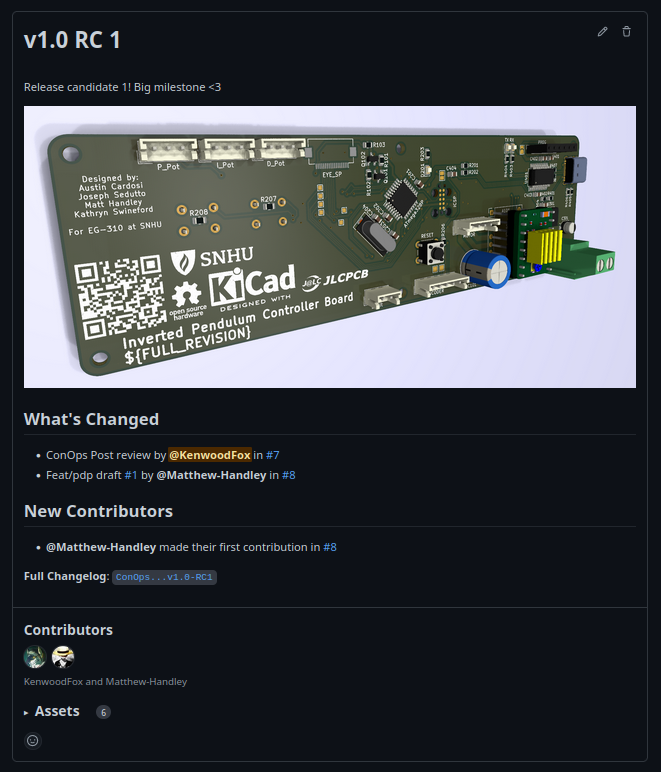
\includegraphics[height=10cm]{v1.0 RC 1}
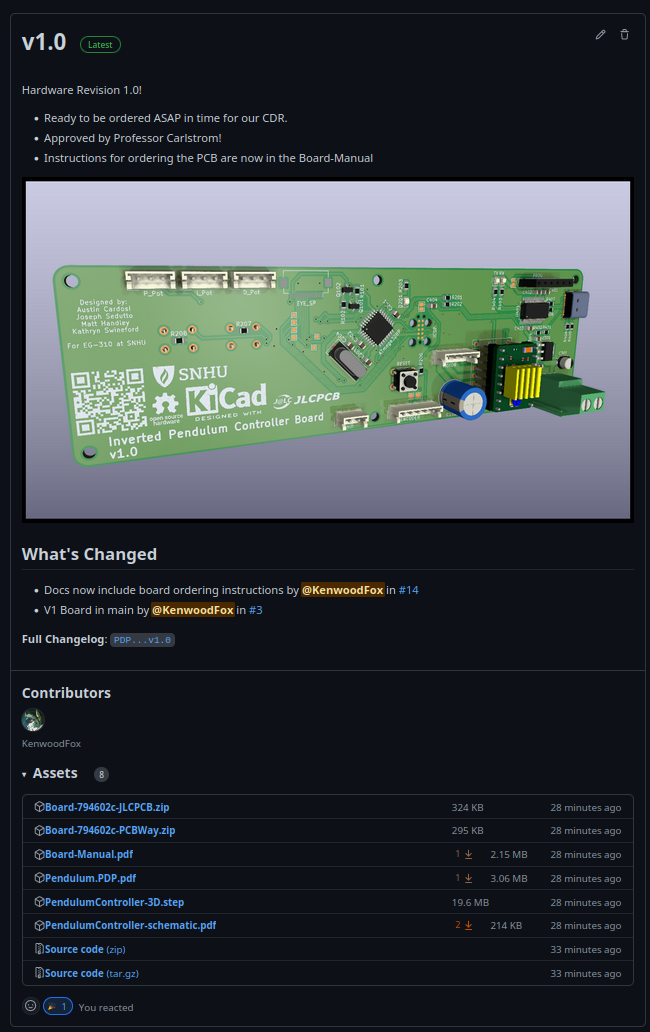
\includegraphics[height=10cm]{v1.0}

\end{document}
